\section{Experimental Results}
\label{sec:expresults}
This section presents experimental results obtained applying Euclidean and Riemannian distances in SSVEP classification task. 
%The performances are compared with LDA. 
The first part of this section describes the data used and the second part provides the assessment of the classification for the considered distances and divergences. %classifications accuracies obtained. 

\subsection{SSVEP Dataset}
The experimental study is conducted on multichannel EEG signals recorded during an SSVEP-based BCI experiment~\cite{kalunga_hybrid_2014}.   
EEG are recorded on $\dc=$ 8 channels from 12 subjects.
The subjects are presented with $\dF=$ 3 visual target stimuli blinking respectively at 13Hz, 21Hz and 17Hz. %$\text{freq}=$
It is a $\dK=$ 4 classes setup combining $\dF=$ 3 stimulus classes and one resting class (no-SSVEP).
In a session, 32 trials are recorded: 8 for each visual stimulus and 8 for the resting class. 
The number of sessions recorded per subject varies from 2 to 5.
For each subject, a test set is made of 32 trials while the remaining trials (which might vary from 32 to 128) make up for the training set.

\subsection{Results and Discussion}

\iflatexml\else \changes{ \fi
Discuss the invariance to right- and left-multiplication by positive matrices. It brings a significant advantage over Euclidean metrics, in terms of electrode placement and unforseen displacement in electrodes position, and can even alleviate anatomical differences.
\iflatexml\else } \fi
\begin{figure}[h!]
\centering
\subfigure[]{
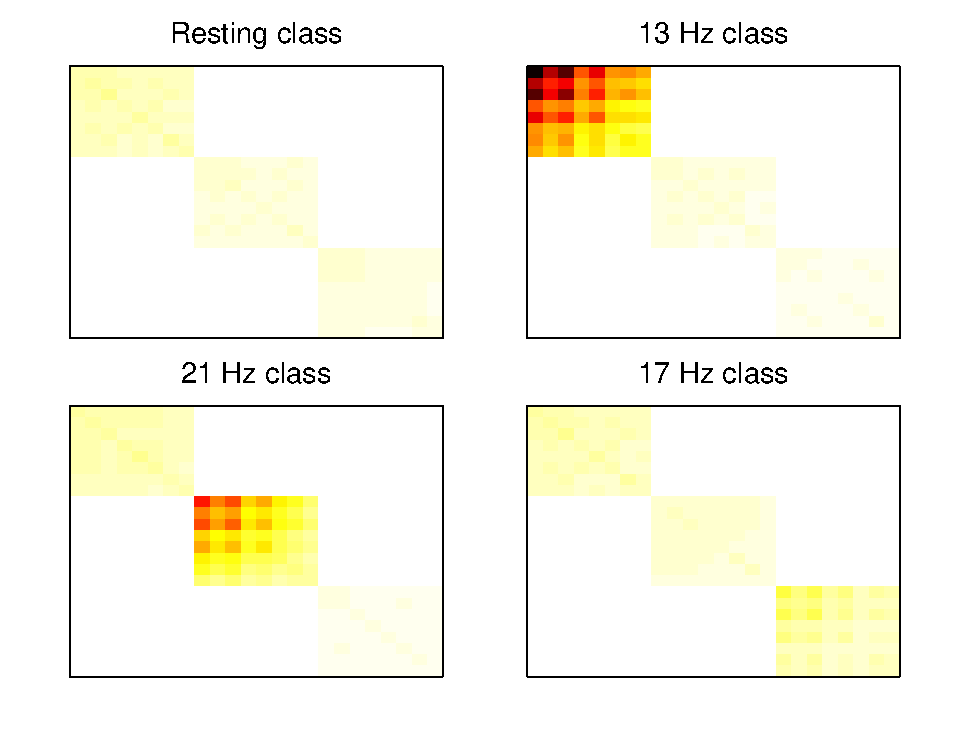
\includegraphics[width=0.47\textwidth]{Figures/covmat.eps}
\label{fig:covmat12}}
\subfigure[]{
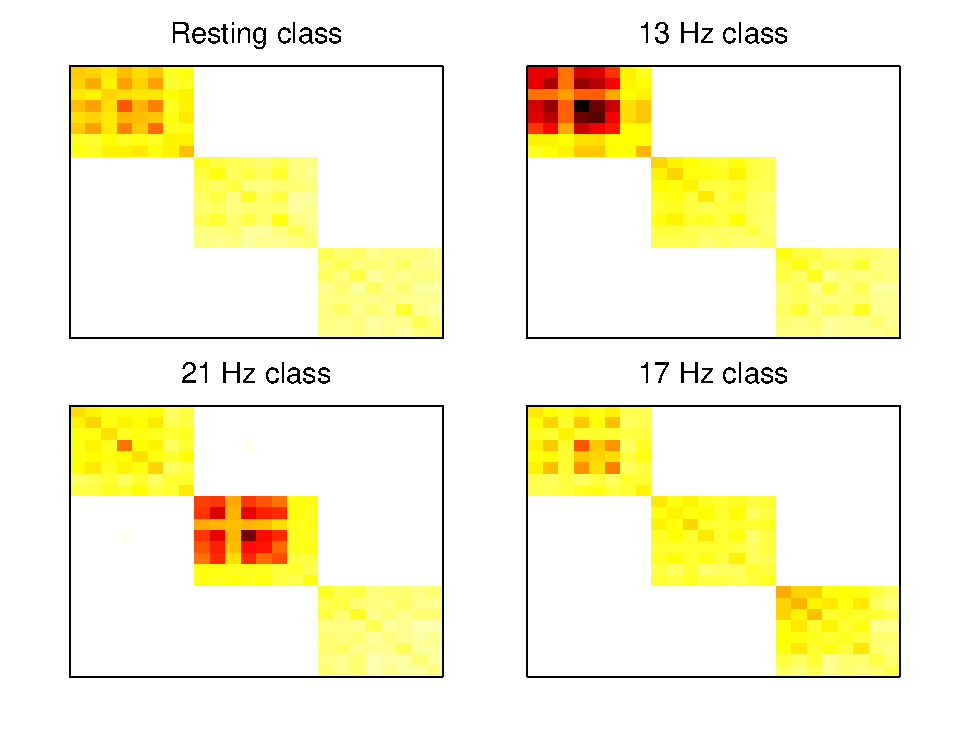
\includegraphics[width=0.47\textwidth]{Figures/covmat11.eps}
\label{fig:covmat11}}
\caption{Representation of covariance matrices: each image is the covariance matrix mean $\Pm^{(\ci)}$ of the class $\ci$, for one session of the recording. The diagonal blocks show the covariance in different frequency bands, i.e. 13Hz in the upper-left block, 21Hz in the middle, and 17Hz in the bottom-right. Subjects with highest (a) and lowest (b) BCI performance. 
}
\label{fig:covmat}
\end{figure}

% The MDM classifier is simple. Once the covariance matrices have been estimated, the only major calculations involved are the mean and distance computations.
The covariance matrices obtained from SSVEP data extended with Eq.~\eqref{eq:ext_data} have interesting features, allowing the discrimination between signals of identical sources but with different frequencies. 
Fig.~\ref{fig:covmat} shows the $K$ classes mean covariance matrices $\Pm^{(\ci)}$ from subjects with the highest (a) and lowest (b) classification accuracies. 
The three 8$\times$8 diagonal blocks hold the covariance matrices of the $\dF=3$ target frequencies.
Inter-frequencies covariances blocks are almost null.
In each mean covariance matrix, the block holding the covariance of the target frequency has the largest values. 
For the resting class, all $\dF$ blocks tend to have similar and small values. These features are more visible in the subject with the highest classification accuracy, and less visible in the one with lowest classification accuracy. 
It is interesting to see that features used for classification have a physiological meaning allowing an intuitive understanding, as opposed to \emph{black-boxes} approaches such as LDA or SVM. EEG processing complexity is encoded by the distance and not by machine learning.
% Contrary to discriminative classifiers classically used in BCI, such as LDA, SVM, etc, which appear as \emph{black-boxes} with difficult interpretation, it is very interesting to see that the presented covariance based classifier is based on features with an easy representation, and thus an intuitive understanding: the observed covariance matrices have a physiological meaning/interpretation.

Based on those covariance matrices, the different distances and means of Table~\ref{tab:dist} are compared in terms of classification accuracy and average CPU time elapsed on a trial classification, which involves the computation of 4 means of class and a distance to each mean.
Table~\ref{tab:res} summarizes results obtained for each subject and each distance/divergence.
Euclidean distance yields drastically low accuracy. 
This support the fact that using Euclidean distance and Arithmetic mean on SPD matrices is not appropriate. 
This is generally attributed to the invariance under inversion and the fact that the determinant of the Arithmetic mean of SPD matrices can be larger than the determinant of its parts; it is referred to as the \textit{swelling effect}.
Since the value of the determinant is a direct measure of dispersion of the multivariate variables (i.e. EEG channels and frequency bands), it leads to poor discrimination in the classification task. 
The swelling effect of Arithmetic mean is shown in Fig.~\ref{fig:swel}: the determinant of the Arithmetic mean is strictly larger than other means, the Log-Euclidean, Affine-Invariant and Bhattacharyya ones yielding similar determinants, close to trials values.

%\begin{sidewaystable}[t]
\begin{table*}[t]
\centering
%\ra{1}
\noindent\adjustbox{max width=\textwidth}{
\begin{tabular}{c|c|c|c|c|c|c||c|c|c|c|c|c|c|c|c|c|c|c|c|c|}
\cline{2-21}
& \multicolumn{6}{ c||}{Euclidean} & \multicolumn{14}{ c| }{Riemannian} \\ \cline{2-21}
& \multicolumn{2}{ c|}{Arithmetic}& \multicolumn{2}{ c|}{Harmonic}& \multicolumn{2}{ c||}{Geometric}&\multicolumn{2}{c|}{Log-Euclidean}&\multicolumn{2}{c|}{Affine-invariant}&\multicolumn{2}{c|}{$\alpha$-divergence}&\multicolumn{2}{c|}{Bhattacharyya}&\multicolumn{2}{c|}{Kullback-Leibler}&\multicolumn{2}{c|}{S-divergence}&\multicolumn{2}{c|}{Wassestein} \\ \cline{1-21}
\multicolumn{1}{ |c| }{Sub.} & acc (\%) & time(s)& acc (\%) & time(s)& acc (\%) & time(s)& acc (\%) & time(s)& acc (\%) & time(s)& acc (\%) & time(s)& acc (\%) & time(s)& acc (\%) & time(s) & acc (\%) & time(s) & acc (\%) & time(s)\\ \hline
\multicolumn{1}{ |c| }{1} & 53.12 & 0.025 & 48.44 & 0.015 & 54.69  &  0.020 & 71.88 & \textbf{0.150}& \textbf{73.44}& 0.194 & 			59.37 & 0.155 & 			68.75 & 			0.225 & 53.12 & 0.030 &  68.75  &  0.220  &  54.69  &  0.630\\ \hline
\multicolumn{1}{ |c| }{2} & 43.75 & 0.020 & 31.25 & 0.025 & 48.44  &  0.020 & 78.13 & 		0.160 & 			79.69 & 0.190 &			79.69 & 0.200 & \textbf{81.25} & \textbf{0.065} & 54.69 & 0.045 & 81.25  &  0.255  &  54.69  &  0.285\\ \hline
\multicolumn{1}{ |c| }{3} & 67.19 & 0.020 & 67.19 & 0.015 & 71.88  &  0.030 & 85.94 & 		0.120 &  		85.93 & 0.205 & \textbf{95.31} & 0.155 & 			85.94 & \textbf{0.100} & 71.88 & 0.060 & 85.94  &  0.200  &  76.56  &  0.280\\ \hline
\multicolumn{1}{ |c| }{4} & 54.68 & 0.030 & 42.19 & 0.010 & 53.12  &  0.020 & 84.38 & 		0.225 &  		87.50 & 0.315 & \textbf{89.07} & 0.250 & 			85.94 & \textbf{0.100} & 48.44 & 0.025 & 85.94  &  0.120  &  65.62  &  0.310\\ \hline
\multicolumn{1}{ |c| }{5} & 37.50 & 0.020 & 26.56 & 0.015 & 39.06  &  0.020 & 62.50 & \textbf{0.115}&  		68.75 & 0.290 & \textbf{73.44} & 0.140 & 			65.62 & 			0.125 & 67.19 & 0.030 & 65.63  &  0.110  &  45.31  &  0.660\\ \hline
\multicolumn{1}{ |c| }{6} & 34.37 & 0.015 & 39.06 & 0.020 & 31.25  &  0.020 & 84.38 & 		0.120 & 			85.94 & 0.210 & \textbf{87.50} & 0.145 & 			82.81 & \textbf{0.100} & 62.50 & 0.030 & 82.81  &  0.130  &  53.13  &  0.300\\ \hline
\multicolumn{1}{ |c| }{7} & 60.42 & 0.027 & 47.92 & 0.013 & 56.25  &  0.017 & 87.50 & 		0.267 &  		88.54 & 0.410 & \textbf{91.66} & 0.417 & 			86.46 & \textbf{0.137} & 54.17 & 0.043 & 86.46  &  0.243  &  69.79  &  0.777\\ \hline
\multicolumn{1}{ |c| }{8} & 67.19 & 0.035 & 68.75 & 0.015 & 82.81  &  0.020 & 90.63 & 		0.215 & \textbf{92.19} & 0.290 & \textbf{92.19} & 0.290 &  \textbf{92.19}& \textbf{0.125} & 71.88 & 0.050 & 92.19  &  0.165  &  85.94  &  0.335\\ \hline
\multicolumn{1}{ |c| }{9} & 57.81 & 0.035 & 42.19 & 0.015 & 59.38  &  0.020 & 70.31 &  		0.275 & 			70.31 & 0.380 & \textbf{75.00} & 0.300 & 			67.19 & \textbf{0.134} & 60.94 & 0.050 & 67.19  &  0.160  &  62.50  &  0.310\\ \hline
\multicolumn{1}{ |c| }{10} & 38.28 & 0.035 & 28.12 & 0.013 & 35.16  &  0.020 & 75.00 & 		0.254 & 			80.47 & 0.514 & \textbf{82.03} & 0.510 & 			78.13 & \textbf{0.160} & 67.97 & 0.028 & 78.13  &  0.263  &  51.56  &  0.650\\ \hline
\multicolumn{1}{ |c| }{11} & 48.44 & 0.025 & 46.88 & 0.010 & 42.19  &  0.025 & 60.94 & 		0.144 & 			65.63 & 0.235 & 			57.81 & 0.150 &  \textbf{75.00}& \textbf{0.105} & 39.06 & 0.040 & 75.00  &  0.195  &  56.25  &  0.575\\ \hline
\multicolumn{1}{ |c| }{12} & 71.25 & 0.032 & 53.75 & 0.022 & 41.25  &  0.024 & 96.25 & \textbf{0.292}& 		96.69 & 0.534 & 			95.62 & 0.634 &  \textbf{96.88} & 		0.300 & 76.88 & 0.042 & 96.88  &  0.466  &  82.50  &  1.042\\ \hline \hline
\multicolumn{1}{ |c| }{\textbf{Avg.}} & 52.83 & 0.027 & 45.19 & 0.016 & 51.29  &  0.021 & 78.98 & 0.194 & 81.27 & 0.314 & \textbf{81.56} & 0.279 & 80.51 & \textbf{0.140} & 60.72 & 0.039 & 80.51 &   0.210 & 63.21 & 0.513\\ \hline
\end{tabular}
}
\caption{Subject classification accuracies (acc(\%)) and average CPU time (time(s)) elapsed for the classification of a single trial. Classification is performed with MDM using either Euclidean or Riemannian means (see Table~\ref{tab:dist}).}
\label{tab:res}
\end{table*}
%\end{sidewaystable}

%\begin{sidewaystable}[t]
%%\begin{table*}[t]
%\centering
%%\ra{1}
%\begin{tabular}{c|c|c||c|c|c|c|c|c|c|c|}
%\cline{2-11}
%& \multicolumn{2}{ c||}{Euclidean} & \multicolumn{8}{ c| }{Riemannian} \\ \cline{2-11}
%& \multicolumn{2}{ c||}{Arithmetic}&\multicolumn{2}{c|}{Log-Euclidean}&\multicolumn{2}{c|}{Affine-invariant}&\multicolumn{2}{c|}{$\alpha$-divergence}&\multicolumn{2}{c|}{Bhattacharyya} \\ \cline{1-11}
%\multicolumn{1}{ |c| }{Sub.} & acc (\%) & time(s)& acc (\%) & time(s)& acc (\%) & time(s)& acc (\%) & time(s)& acc (\%) & time(s)\\ \hline
%\multicolumn{1}{ |c| }{1} & 53.12 & 0.025 & 71.88 & \textbf{0.150} & \textbf{73.44} & 0.194 & 59.37 & 0.155 & 68.75 & 0.225\\ \hline
%\multicolumn{1}{ |c| }{2} & 43.75 & 0.020 & 78.13 & 0.160 & 79.69 & 0.190 & 79.69 & 0.200 & \textbf{81.25} & \textbf{0.065}\\ \hline
%\multicolumn{1}{ |c| }{3} & 67.19 & 0.020 & 85.94 & 0.120 &  85.93 & 0.205 & \textbf{95.31} & 0.155 & 85.94 & \textbf{0.100}\\ \hline
%\multicolumn{1}{ |c| }{4} & 54.68 & 0.030 & 84.38 & 0.225 &  87.50 & 0.315 & \textbf{89.07} & 0.250 & 85.94 & \textbf{0.100}\\ \hline
%\multicolumn{1}{ |c| }{5} & 37.50 & 0.020 & 62.50 & \textbf{0.115} &  68.75 & 0.290 & \textbf{73.44} & 0.140 & 65.62 & 0.125\\ \hline
%\multicolumn{1}{ |c| }{6} & 34.37 & 0.015 & 84.38 & 0.120 & 85.94 & 0.210 & \textbf{87.50} & 0.145 & 82.81 & \textbf{0.100}\\ \hline
%\multicolumn{1}{ |c| }{7} & 60.42 & 0.027 & 87.50 & 0.267 &  88.54 & 0.410 & \textbf{91.66} & 0.417 & 86.46 & \textbf{0.137}\\ \hline
%\multicolumn{1}{ |c| }{8} & 67.19 & 0.035 & 90.63 & 0.215 & \textbf{92.19} & 0.290 & \textbf{92.19} &  0.290 & \textbf{92.19} & \textbf{0.125}\\ \hline
%\multicolumn{1}{ |c| }{9} & 57.81 & 0.035 & 70.31 &  0.275 & 70.31 & 0.380 & \textbf{75.00} & 0.300 & 67.19 & \textbf{0.134}\\ \hline
%\multicolumn{1}{ |c| }{10} & 38.28 & 0.035 & 75.00 & 0.254 & 80.47 & 0.514 & \textbf{82.03} & 0.510 & 78.13 & \textbf{0.160}\\ \hline
%\multicolumn{1}{ |c| }{11} & 48.44 & 0.025 & 60.94 & 0.144 & 65.63 & 0.235 & 57.81 & 0.150 & \textbf{75.00} & \textbf{0.105}\\ \hline
%\multicolumn{1}{ |c| }{12} & 71.25 & 0.032 & 96.25 & \textbf{0.292} & 96.69 & 0.534 & 95.62 & 0.634 & \textbf{96.88} & 0.300\\ \hline \hline
%\multicolumn{1}{ |c| }{\textbf{Avg.}} & 52.83 & 0.027 & 78.98 & 0.194 & 81.27 & 0.314 & \textbf{81.56} & 0.279 & 80.51 & \textbf{0.140}\\ \hline
%\end{tabular}
%\caption{Subject classification accuracies (acc(\%)) and average CPU time (time(s)) elapsed for the classification of a single trial. Classification is performed with MDM using either Euclidean or Riemannian means (see Table~\ref{tab:dist}).}
%\label{tab:res}
%%\end{table*}
%\end{sidewaystable}

\begin{figure}[h!]
\centering
\subfigure[]{
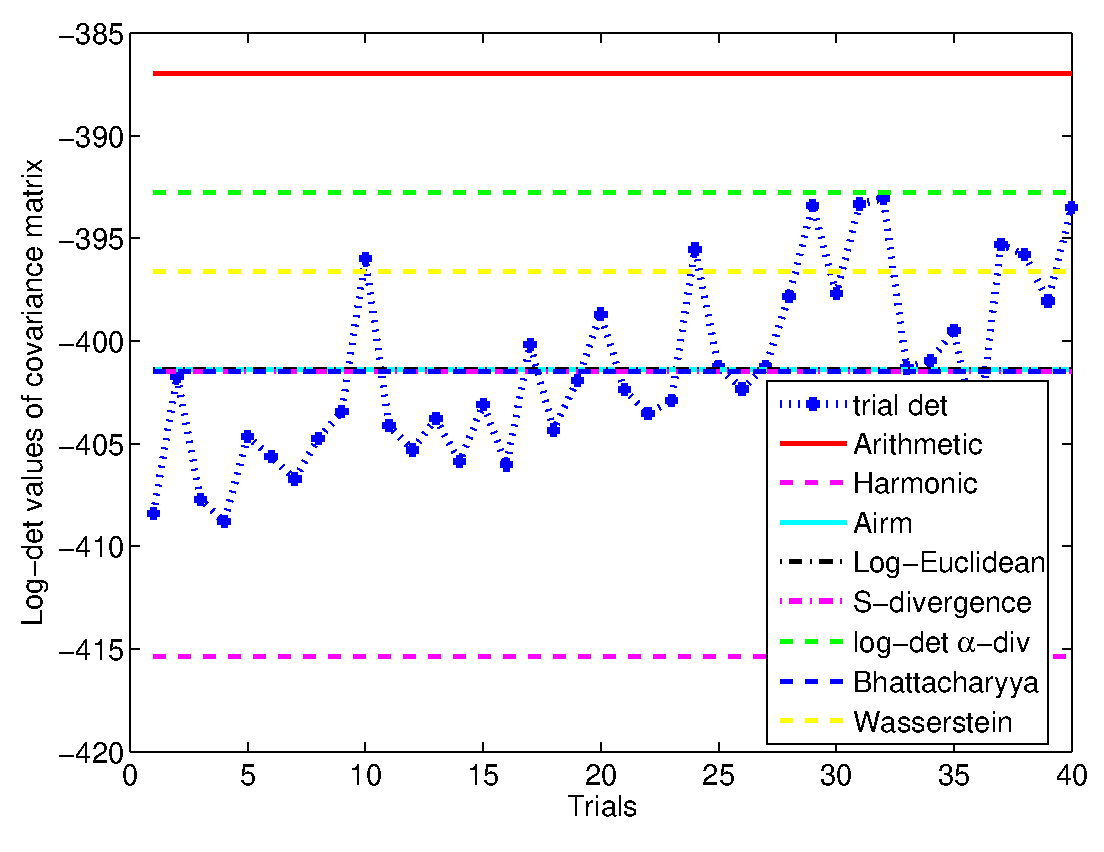
\includegraphics[width=0.46\textwidth]{Figures/swel.eps}
\label{fig:swel}
}
\subfigure[]{
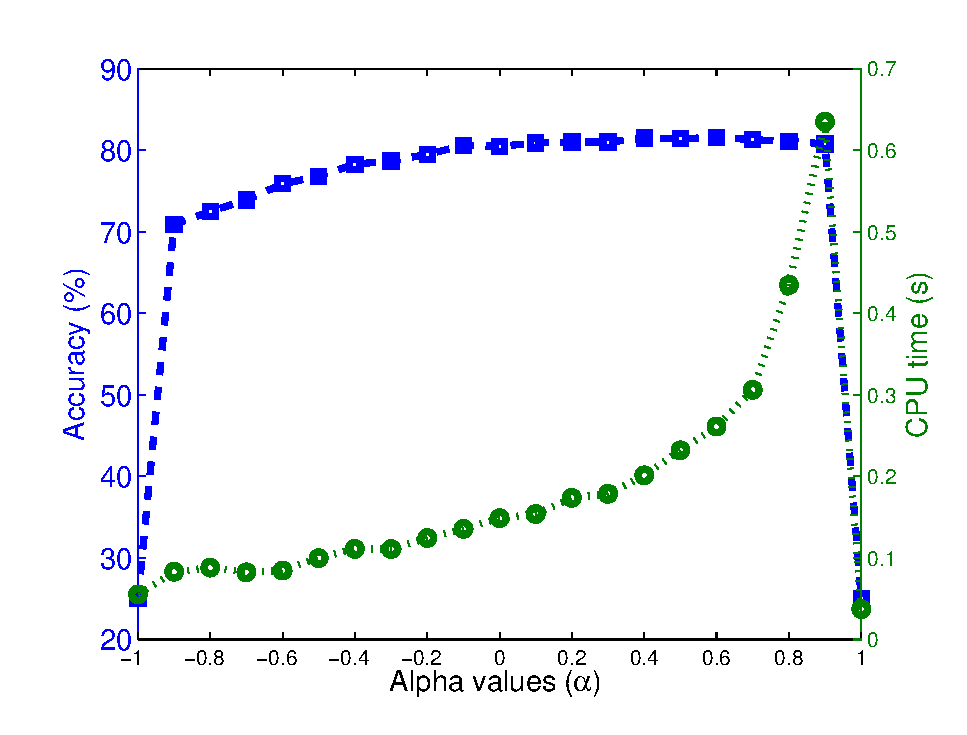
\includegraphics[width=0.49\textwidth]{Figures/alpha_cross.eps}
\label{fig:alphacross}
}
\caption{(a): Swelling effect of Arithmetic mean shown through log-determinant values. Training trials are taken from the 13Hz class of the subject with the highest BCI performance. Log-determinant values are given for each trial covariance (points), and for means of Table~\ref{tab:dist} (horizontal lines). (b): Classification accuracy and CPU time, obtained with $\alpha$-divergence for $-1\leqslant \alpha  \leqslant 1$.} 
\label{fig:swel_alpha}
\end{figure} 

Riemannian distances significantly improve classification performances, with $\alpha$-divergence yielding the best results (81.56\%). 
The value of $\alpha$ was set to 0.6 through cross-validation. 
This procedure lasted 225.42 seconds and makes $\alpha$-divergence the most costly method, due to the optimization of its parameter $\alpha$. 
Log-Euclidean yields lower classification accuracy (average 78.98\%) but could be computed faster than $\alpha$-divergence or Affine-Invariant distance.
However, the Bhattacharyya distance has the lowest computational cost of the considered Riemannian distances (average CPU time 0.140s), with a higher average accuracy of 80.51\%. 
So, it is good trade-off between efficiency and speed. 
The accuracies and CPU time of the $\alpha$-divergence at different values of $\alpha$ are shown in Fig.~\ref{fig:alphacross}.
It is seen that for $\alpha = \pm 1$, where $\alpha$-divergence represents a Bregman divergence associated with the log-determinant function, % also known as  log-det divergence, 
the classification accuracy are at the lowest accuracy (25\%). 
For all other values of alpha, the expected accuracy is 78.85$\pm$3.3\% and one can choose $-1 < \alpha < 1$ without any major impact on classification results.
%$\alpha$ could thus be fixed to any value between $\left]-1,+1\right[$ without causing drastic deterioration of accuracy. 
%For instance, the Bhattacharyya mean is equivalent to the $\alpha$-divergence mean with $\alpha$=0. 

This experiment on real EEG data shows that it is crucial to process covariance matrices with dedicated Riemannian tools, impacting the efficiency of the classification. 